\documentclass[a4paper,12pt]{article}
\usepackage[left=0.5cm, right=2cm, top=1cm, bottom=1cm]{geometry}
\usepackage{graphicx}
\usepackage{array}
\usepackage{booktabs}
\usepackage{xcolor} 
\usepackage{physics}
\usepackage{amsmath}
\usepackage{tikz}
\usepackage{mathdots}
\usepackage{yhmath}
\usepackage{cancel}
\usepackage{color}
\usepackage{siunitx}
\usepackage{array}
\usepackage{multirow}
\usepackage{amssymb}
\usepackage{gensymb}
\usepackage{tabularx}
\usepackage{extarrows}
\usepackage{booktabs}
\usetikzlibrary{fadings}
\usetikzlibrary{patterns}
\usetikzlibrary{shadows.blur}
\usetikzlibrary{shapes}
\usepackage{pgfplots}

\newcommand{\emptybox}[1]{\framebox[1cm][c]{\rule{0pt}{#1pt}}}
\newcommand{\ans}[1]{\underline{\makebox[1.5cm][c]{\textcolor{green}{#1}}}}
\usepackage{keyval}

\makeatletter
\define@key{datastats}{data}{\def\ds@data{#1}}
\define@key{datastats}{mean}{\def\ds@mean{#1}}
\define@key{datastats}{median}{\def\ds@median{#1}}
\define@key{datastats}{mode}{\def\ds@mode{#1}}

\newcommand{\datastats}[1]{%
  \setkeys{datastats}{#1}
  \parbox[t]{\linewidth}{
      \vspace{0.1cm}
        \centering  \text{\ds@data}\\
    \flushleft Mean : \ans{\ds@mean} \\
    Median: \ans{\ds@median} \\
    Mode : \ans{\ds@mode}\\[6pt]
  }%
}

\newcommand{\picstats}[2]{%
  \begin{center}
    \begin{tikzpicture}[x=0.75pt,y=0.75pt,yscale=-1,xscale=1]
    \foreach \g [count=\i from 0] in {#1} {
      \pgfmathsetmacro{\x}{81 + 86*\i}
      \draw (\x, 107) node {
\includegraphics[width=52.5pt,height=52.5pt]{Task 4/images/apple.jpg}};
      \draw (\x-17, 103) node [anchor=north west][inner sep=0.75pt]   [align=left] {\g g};
    }
    \end{tikzpicture}
  \end{center}
  \flushleft Median of apples = \ans{#2}%
}

\newcommand{\tempstats}[2]{%
  \begin{center}
    \begin{tikzpicture}[x=0.75pt,y=0.75pt,yscale=-1,xscale=1]
    \foreach \temp [count=\i from 0] in {#1} {
      \pgfmathsetmacro{\x}{53.5 + 70*\i}
      \draw (\x, 67.5) node {
\includegraphics[width=27.75pt,height=44.25pt]{Task 4/images/temp.jpg}};
      \draw (\x + 10.5, 51) node [anchor=north west][inner sep=0.75pt] [align=left] {\temp ℃};
    }
    \end{tikzpicture}
  \end{center}
  \flushleft The average (mean) of the recorded temperatures = \ans{#2\,$^\circ$C}%
}

\newcommand{\sportbar}[3]{%
  \begin{minipage}[t]{0.13\textwidth}
    \centering
    \foreach \i in {1,...,#2} {
      \includegraphics[width=0.9cm]{Task 4/images/#3}\\[-2pt]
    }
    \vspace{2pt}
    {\footnotesize #1}
  \end{minipage}
}

\newcommand{\answer}[1]{%
    \begin{center}
    \textcolor{green}{\textbf{#1}}\par
    \end{center}
}
\definecolor{colorone}{rgb}{0.1, 0.1, 0.8}
\definecolor{colortwo}{rgb}{0.8, 0.1, 0.1}
\newcommand{\StudentBarPlot}[2]{%
	\begingroup
	\addplot+[ 
	style={pattern=dots, pattern color=#1},
	draw=black 
	] coordinates {#2};
	\endgroup
}
\makeatother


\begin{document}
    
	\setlength{\fboxrule}{2pt}
	\fbox{% 
		\begin{minipage}{\dimexpr\textwidth-2\fboxsep-2\fboxrule\relax}
			\textbf{Topic Name: Data handling}\\
            \textbf{\underline{Section name:} Measures of central tendency}
			
			\vspace{0.3cm}
			1. Calculate the mean, median and mode for the given datasets.
			
			\vspace{0.3cm}
			\begin{tabular}{|p{0.48\textwidth}|p{0.48\textwidth}|}
              \hline
              \datastats{data={1, 2, 3, 4, 5, 6, 7}, mean=4, median=4, mode=-} &
              \datastats{data={17, 21, 42, 35, 16, 21, 5}, mean=22.4, median=21, mode=21} \\
              \hline
              \datastats{data={15, 13, 12, 11, 11, 9, 7, 6}, mean=10.5, median=11, mode=11} &
              \datastats{data={44, 48, 44, 46, 47, 44, 42, 44}, mean=44.8, median=44, mode=44} \\
              \hline
              \datastats{data={5, 4, 5, 6, 5, 4, 6, 4, 5, 2, 7}, mean=4.91, median=5, mode=5} &
              \datastats{data={1.6, 3.2, 4.8, 5.7, 6.3, 7.6, 8.4, 9.5}, mean=5.88, median=6, mode=-} \\
              \hline
            \end{tabular}
			
			\vspace{0.3cm}
			2. Find the median of the given apples.
            
            \begin{center}
                \picstats{500, 75, 120, 180, 160, 50}{140}
    	    \end{center}
            \vspace{0.5cm}

            3. Find the average temperature recorded in the city over period of week.
            \tempstats{32, 28, 26, 22, 33, 32, 25}{28.2}
            
        4. Find the mode of the given banana set.\\
        \begin{center}
        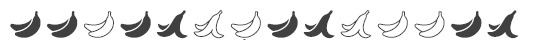
\includegraphics[width=15cm]{Task 4/images/4ques.jpg}\\
        \end{center}
        The mode of the given bananas is \ans{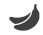
\includegraphics[width=1.5cm]{Task 4/images/4ans.jpg}}
		\end{minipage}
	}
    \newpage

\fbox{%
\begin{minipage}{\dimexpr\textwidth-2\fboxsep-2\fboxrule\relax}
  \section*{\textbf{\underline{Section name:} Representation of data (Bar graph)}}
  In a class of 7th-grade students, a survey was conducted to determine their favorite sports. The results of the survey are displayed in the bar graph. Represent the given data in the table and answer the following questions.

  \begin{center}
    \textbf{Sports Choices: Class 7 Preferences}
  \end{center}

  \begin{center}
  \begin{tikzpicture}
  \draw[->] (-0.5,0) -- (-0.5,6.5); 
  \foreach \y in {0,5,...,40} {
    \pgfmathsetmacro{\scaledY}{\y*0.15} 
    \draw[gray!70] (-0.5,\scaledY) -- (9,\scaledY); 
    \node[left] at (-0.5,\scaledY) {\small \y}; 
  }
  \node[rotate=90, anchor=south] at (-1.2,3) {\textbf{No. of students}}; 

  \draw[->] (-0.5,0) -- (9,0); 
  \node at (4.25,-1.0) {\textbf{Sports}};

  \foreach \x/\count/\img/\label in {
    0.5/15/basketball.png/Basketball,
    2.0/40/cricket.jpg/Cricket,
    3.5/35/tennis.png/Tennis,
    5.0/30/swimming.png/Swimming,
    6.5/25/chess.png/Chess,
    8.0/10/baseball.png/Baseball} {

    \pgfmathsetmacro{\maxY}{40} 
    \pgfmathsetmacro{\numImages}{int(\count / 5)} 
    
    \foreach \i in {1,...,\numImages} {
      \pgfmathsetmacro{\imageY}{(\i - 0.5) * 0.75} 
      \node at (\x, \imageY) {\includegraphics[height=0.8cm]{Task 4/images/\img}};
    }
    \node[align=center, font=\footnotesize] at (\x, -0.4) {\label};
  }
\end{tikzpicture}
  \end{center}
   \begin{center}
	\renewcommand{\arraystretch}{1.5}
	\begin{tabular}{|c|c|c|c|c|c|c|}
		\hline
		\textbf{Types of sports} & Basketball & Cricket & Tennis & Swimming & Chess & Baseball \\
		\hline
		\textbf{No of students} & 
		\textcolor{green}{\textbf{15}} & 
		\textcolor{green}{\textbf{40}} & 
		\textcolor{green}{\textbf{35}} & 
		\textcolor{green}{\textbf{30}} & 
		\textcolor{green}{\textbf{25}} & 
		\textcolor{green}{\textbf{10}} \\
		\hline
	\end{tabular}
    \end{center}
    \vspace{0.3cm}
    \begin{enumerate}
    	\item In Y-axis, 1 unit = \ans{5} number of students.
    	\item Which sport is the most popular among the students? \ans{Cricket}
    	\item How many more students prefer chess compared to Basketball? \\
        \textcolor{green}{10 students}
    	\item If each student can select only one favorite sport, then find the total number of students surveyed for class 7\textsuperscript{th}. \\
        \textcolor{green}{155 students}
    	\item Assume there are 200 students in class, if each student can only choose one favorite sport, how many students did not select any of the listed sports? \\ 
        \textcolor{green}{45 students}
    \end{enumerate}
\end{minipage}
}
\newpage
\fbox{
    \begin{minipage}{\dimexpr\textwidth-2\fboxsep-2\fboxrule\relax}
    \section*{\textbf{\underline{Section name:} Representation of data (Double bar graph)}}
    The below double bar graph shows the scores achieved by the students before and after completing the Learn Basics course. Observe the given bar graph and answer the questions given below.
    \begin{center}
		\textbf{Students test performance before and after Learn Basics}\\[10pt]

		\begin{tikzpicture}
		\begin{axis}[ 
			width=15cm, 
			height=10cm, 
			ybar=0pt, 
			bar width=20pt, 
			enlarge x limits=0.1, 
			symbolic x coords={Karthi, Baviya, Kavipriya, Kavinya, Saran, Pradeepa}, 
			xtick=data, 
			ylabel={Test score}, 
			xlabel={Students}, 
			legend style={at={(0.5,1.15)}, anchor=south, legend columns=-1}, 
			ymin=0, ymax=100, 
			axis lines=left, 
			axis line style={draw=black}, 
			enlarge x limits=0.1, 
			]
			
			\StudentBarPlot{colorone}{(Karthi,50) (Baviya,60) (Kavipriya,40) (Kavinya,80) (Saran,25) (Pradeepa,50)}

			\StudentBarPlot{colortwo}{(Karthi,80) (Baviya,70) (Kavipriya,75) (Kavinya,95) (Saran,85) (Pradeepa,60)}
			
			\legend{Before Learn Basics, After Learn Basics}
		\end{axis}
	\end{tikzpicture}
		
		\vspace{0.5cm}
		\begin{tabular}{|l|*6{c|}}
			\hline
			\textbf{Students} & \textbf{Karthi} & \textbf{Baviya} & \textbf{Kavipriya} & \textbf{Kavinya} & \textbf{Saran} & \textbf{Pradeepa} \\
			\hline
			\textbf{Before LB} & 50 & 60 & 40 & 80 & 25 & 50 \\
			\hline
			\textbf{After LB} & 80 & 70 & 75 & 95 & 85 & 60 \\
			\hline
		\end{tabular}
	\end{center}
    
    \begin{enumerate}
		\item \textbf{Who scored the lowest marks before completing the Learn Basics course?}\\
		\answer{Saran}
		
		\item \textbf{Which student secured the highest mark after completing the Learn Basics course?}\\
		\answer{Kavinya}
		
		\item \textbf{If the passing grade for the test is 70, how many students passed the test after attending a course from Learn Basics?}\\
		\answer{5 students}
		
		\item \textbf{Calculate the average score before and after the tests for all the students together.}\\
		\answer{Average score before LB: 50.8 \\ Average score after LB: 77.5}
	\end{enumerate}
    \end{minipage}
}
\end{document}
